% Local model tooling: engine, runtimes and the clients that talk to them.
% ---------------------------------------------------------------------------
% style.tex --- shared preamble for every figure in book/figures/tikz/
%
% One style for all figures: Latin Modern, thin black lines, a light grey
% fill, and one accent colour used only to mark what is untrusted or wrong.
% Build with scripts/build_figures.sh; see book/figures/README.md.
% ---------------------------------------------------------------------------
\documentclass[tikz,border=6pt]{standalone}
\usepackage[T1]{fontenc}
\usepackage{lmodern}
\usetikzlibrary{arrows.meta,positioning,shapes.geometric,calc,fit,backgrounds}

\hyphenpenalty=10000   % short lines in boxes: ragged, never hyphenated

\definecolor{lightgrey}{gray}{0.92}
\definecolor{accent}{HTML}{9B2D20}

\tikzset{
  every picture/.style={
    line width=0.6pt,
    font=\small,
    >={Stealth[length=5pt,width=4pt]},
    node distance=14pt and 24pt,
  },
  % shapes
  box/.style={draw, rectangle, inner xsep=8pt, inner ysep=5pt,
              minimum height=22pt, align=center},
  grey/.style={box, fill=lightgrey},
  rounded/.style={box, rounded corners=9pt},
  decision/.style={draw, diamond, aspect=2.4, inner sep=1.5pt, align=center},
  group/.style={draw, dashed, rounded corners=5pt, inner sep=7pt},
  % text
  tag/.style={font=\footnotesize, align=center, inner sep=2pt},
  note/.style={font=\footnotesize\itshape, align=center, inner sep=2pt},
  code/.style={font=\small\ttfamily},
  codetag/.style={font=\footnotesize\ttfamily, align=center, inner sep=2pt},
  title/.style={font=\small\scshape, align=center, inner sep=2pt},
  % lines
  arrow/.style={->},
  back/.style={->, dashed},
  thin/.style={line width=0.4pt, gray},
  % the one accent, for what is untrusted, wrong or missing
  bad/.style={accent},
  badbox/.style={box, draw=accent, text=accent},
}

\begin{document}
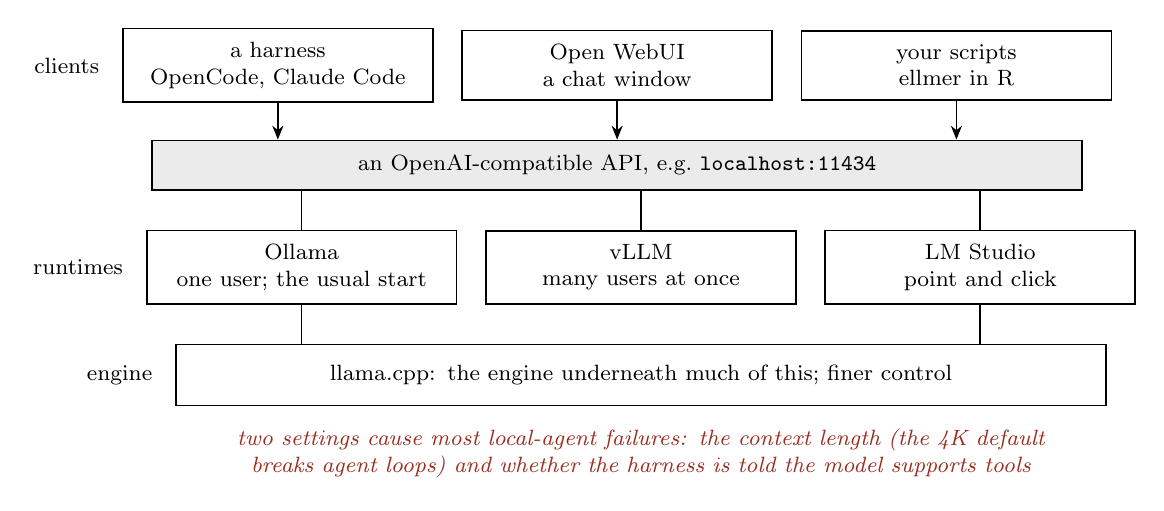
\begin{tikzpicture}[node distance=14pt and 10pt,
                    cell/.style={box, text width=96pt, align=center, font=\footnotesize}]
  % clients
  \node[cell] (harness) at (0,0) {a harness\\OpenCode, Claude Code};
  \node[cell, right=of harness] (webui) {Open WebUI\\a chat window};
  \node[cell, right=of webui] (script) {your scripts\\ellmer in R};
  \node[tag, left=6pt of harness, anchor=east] {clients};
  % API line
  \node[grey, below=of webui, text width=320pt, align=center, minimum height=18pt, inner ysep=3pt, font=\footnotesize]
    (api) {an OpenAI-compatible API, e.g.\ \texttt{localhost:11434}};
  % runtimes
  \node[cell, below=of api, xshift=-114pt] (ollama) {Ollama\\one user; the usual start};
  \node[cell, right=of ollama] (vllm) {vLLM\\many users at once};
  \node[cell, right=of vllm] (lms) {LM Studio\\point and click};
  \node[tag, left=6pt of ollama, anchor=east] {runtimes};
  % engine
  \node[box, below=of vllm, text width=320pt, align=center, font=\footnotesize] (engine) {llama.cpp: the engine underneath much of this; finer control};
  \node[tag, left=6pt of engine, anchor=east] {engine};
  \foreach \c in {harness,webui,script} \draw[->] (\c) -- (\c |- api.north);
  \foreach \r in {ollama,vllm,lms} \draw (\r |- api.south) -- (\r);
  \foreach \r in {ollama,lms} \draw (\r) -- (\r |- engine.north);
  \node[note, below=6pt of engine, text width=330pt, text=accent]
    {two settings cause most local-agent failures: the context length (the 4K default breaks agent loops)
     and whether the harness is told the model supports tools};
\end{tikzpicture}
\end{document}
